\chapter{\textsc{Interfaces séries}}

Les interfaces parallèles ne sont quasiment plus utilisées aujourd'hui à cause du nombre de broches nécessaires et des performances électriques demandées. L'interface série n'utilise que 2 ou 3 broches et bénéficie de meilleur performances. Elles demandent, par contre, plus de matériel et de logiciel pour effectuer la sérialisation et dé-sérialisation.


\section{Notion de pile protocolaire}
Il est utile d'inscrire les interfaces séries au sein des notions de la téléinformatique comme celle de la pile protocolaire. Cette pile permet de découper toutes les opérations nécessaires en couches. Chaque couche à une fonction bien précise et est développée indépendamment des autres. 

\subsection{Modèle OSI (Open Systems Interconnection)}
Le modèle OSI est un modèle théorique d'une pile de communication avec sept couches (fig. \ref{fig:osi}). 

\begin{figure}[htb]
  \centering
  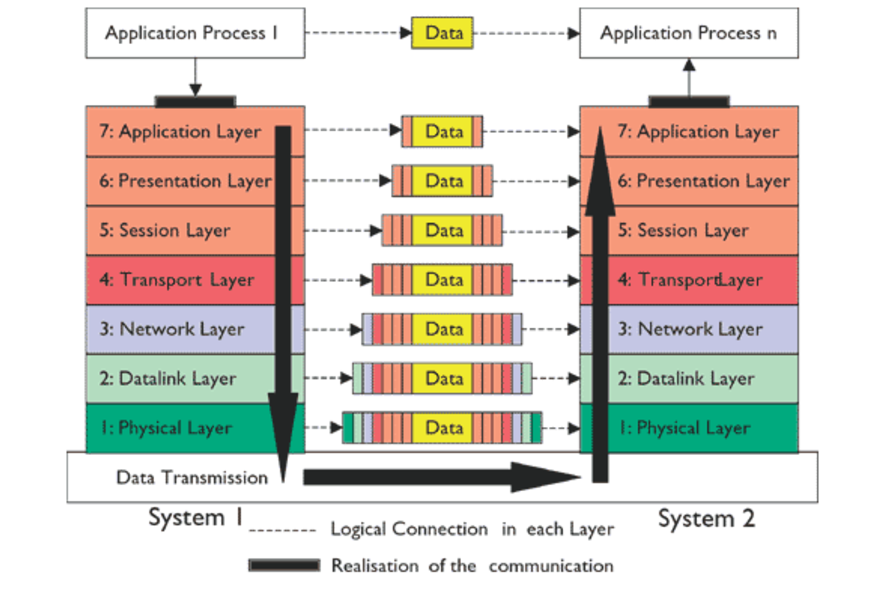
\includegraphics[angle=0, width=10cm]{./Figures/serial/modelOSI.pdf}
  \rule{35em}{0.5pt}
  \caption[osi]{Modèle OSI}
  \label{fig:osi}
\end{figure}

Les couches qui sont nécessaires à l'établissement d'une communication sont les couches 1 à 4. Les autres sont des couches liées aux services et aux applications.

\begin{enumerate}
\item Couche physique: Traite les aspects électriques de la ligne série
\item Couche paquet: Encapsule les données avec des bits de contrôle e.g. pour la détection d'erreurs
\item Couche réseau: Indique la destination (s'il y a plus que deux noeuds sur le réseau)
\item Couche transport: Découpe les données en paquets et gère la retransmission en cas d'erreurs
\end{enumerate}

\subsection{Pile protocolaire IP}
Le protocole IP (Internet Protocol) est simplifié par rapport au modèle OSI (fig. \ref{fig:tcpip}). Il ne contient que quatre couches ce qui parait plus simple mais en pratique n'est pas idéal car il groupe plusieurs fonctions dans une seule couche.

\begin{figure}[htb]
  \centering
  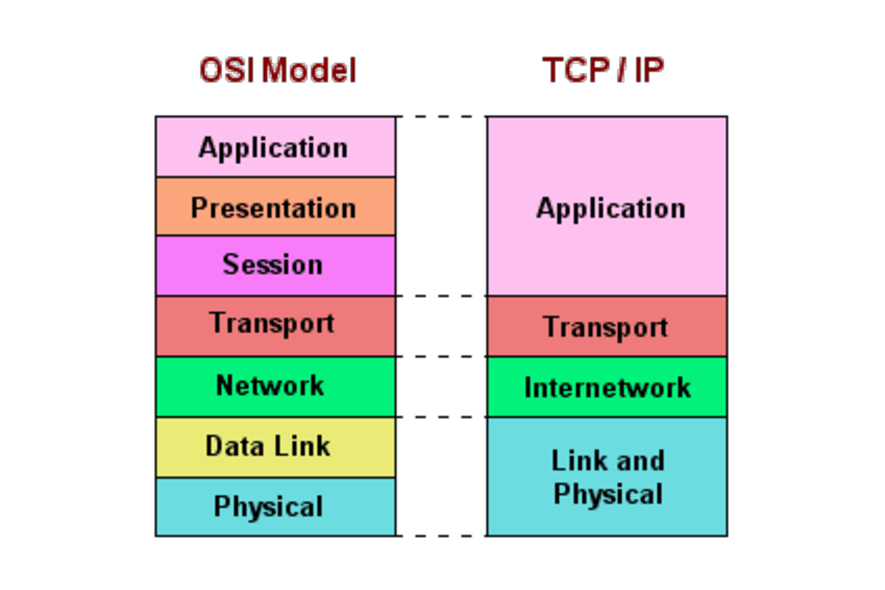
\includegraphics[angle=0, width=10cm]{./Figures/serial/tcpipstack.pdf}
  \rule{35em}{0.5pt}
  \caption[tcpip]{Comparaison des piles protocolaires}
  \label{fig:tcpip}
\end{figure}

\section{UART (Universal Asynchronous Receiver Transmitter)}

Les UART sont des sérialiseurs/désérialiseurs simples. Un UART permet d'implémenter la couche 2 du modèle OSI. L'UART est asynchrone ce qui veut dire qu'il ne propage pas de signal d'horloge de l'émetteur au récepteur. Il est néanmoins aisé d'ajouter une ligne d'horloge pour rendre l'UART synchrone.

\begin{figure}[htb]
  \centering
  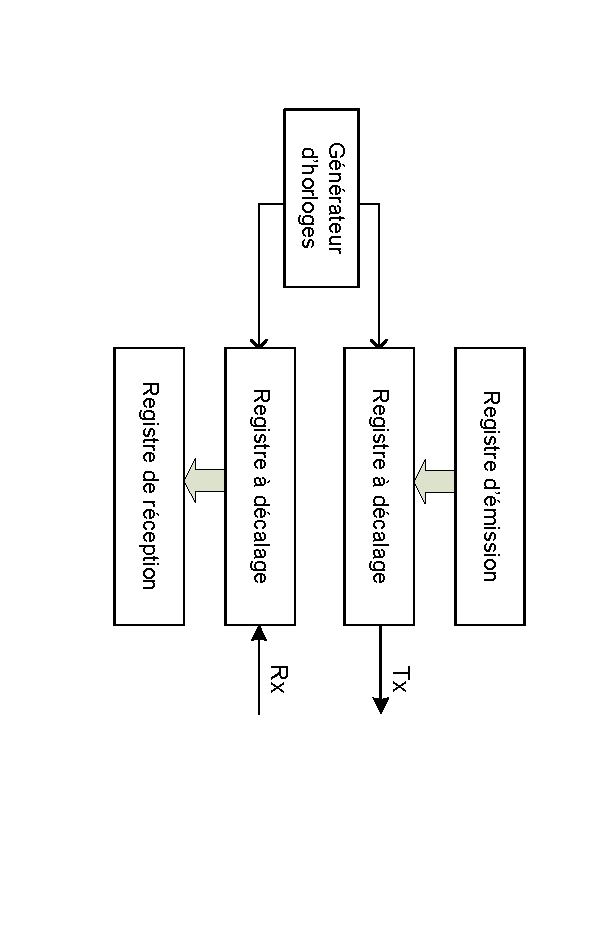
\includegraphics[angle=90, trim = 15mm 0mm 5mm 0mm, clip, width=13cm]{./Figures/serial/UART.pdf}
  \rule{35em}{0.5pt}
  \caption[uart]{Principe de fonctionnement d'une UART}
  \label{fig:uart}
\end{figure}

Au niveau matériel, l'UART est composé de 4 registres dont deux à décalage. Le générateur d'horloge donne la fréquence de transmission ou vitesse de transmission. Du point de vue logiciel on accède à l'UART simplement en écrivant dans le registre d'émission et en lisant le registre de réception.

\subsection{RS-232C}
Historiquement, les interfaces séries étaient très simples d'un point de vue logiciel mais par contre plus compliquées d'un point de vue matériel. C'est le cas de l'interface RS-232C développée en 1969.

La couche physique du RS-232C à néanmoins évolué depuis 1969, par contre la couche 2 est toujours la même. On peut réaliser cette couche 2 avec un UART.

\section{Interface SPI}

Dix ans après la RS-232C, Motorola invente l'interface SPI en 1979. C'est un changement radical, avec une communication synchrone entre les émetteurs et les récepteurs. Ce changement permet d'aller beaucoup plus vite dans la transmission.

\begin{figure}[htb]
  \centering
  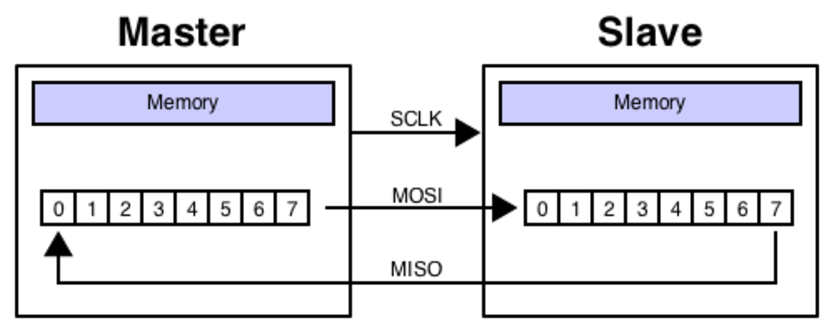
\includegraphics[width=12cm]{./Figures/serial/SPI_8-bit_circular_transfer.pdf}
  \rule{35em}{0.5pt}
  \caption[spi]{Principe de fonctionnement d'une interface SPI}
  \label{fig:spi}
\end{figure}

L'interface SPI utilise deux registres à décalage bouclés. Ceci permet de relire l'information transmise est ainsi vérifier que ce qui a été transmis est bien correcte. Pour écrire ou lire, on utilise le même principe que pour l'UART, c-à-d écrire dans le registre d'émission ou lire le registre de réception.

Il est possible de connecter plusieurs périphériques sur une interface SPI à l'aide de signaux sortant d'un GPIO et allant sur une entrée "chip-select" CS. Il faut juste sélectionner le bon CS depuis le code.

\section{Interface I2C}

Trois ans après la SPI, Philips invente l'interface I2C en 1982. Cette interface amène une innovation majeur qui est la réalisation d'une couche 3 logicielle permettant d'adresser 256 noeuds. On peut donc relier tous les périphériques d'une carte à l'aide d'une interface I2C. Ils sont connectés sur deux lignes communes SDA et SCL:

\begin{figure}[htb]
  \centering
  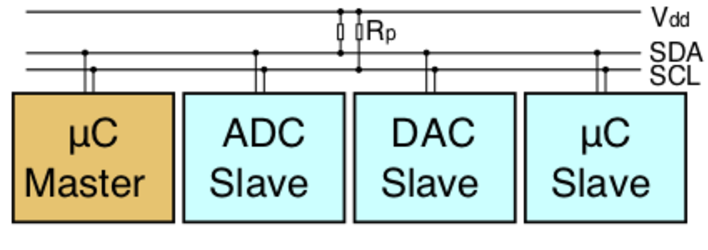
\includegraphics[width=10cm]{./Figures/serial/I2C.pdf}
  \rule{35em}{0.5pt}
  \caption[i2c]{Système avec un bus I2C}
  \label{fig:i2c}
\end{figure}

Les lignes, SDA et SCL, sont tirées vers l'alimentation positive (Vdd) à l'aide de deux résistance pull-up. Elles doivent être dimensionnées par rapport à la vitesse de transmission choisie. Pour sélectionner un périphérique en particulier, il faut connaitre son adresse I2C et la placer dans le registre d'adresse de l'interface.

\section{Interface USB}

L'interface série la plus récente que l'on trouve dans les microcontrôleurs est l'USB (Universial Serial Bus) développée en 1996. Cette interface à comme avantage majeur sur les autres l'utilisation d'une signalisation basse tension différentielle LVDS (Low Voltage Differential Signal). Par contre, cette interface est purement point à point c-à-d qu'elle ne relie qu'un noeud à un autre. De ce fait, elle ne remplace pas les précédentes.

\begin{figure}[htb]
  \centering
  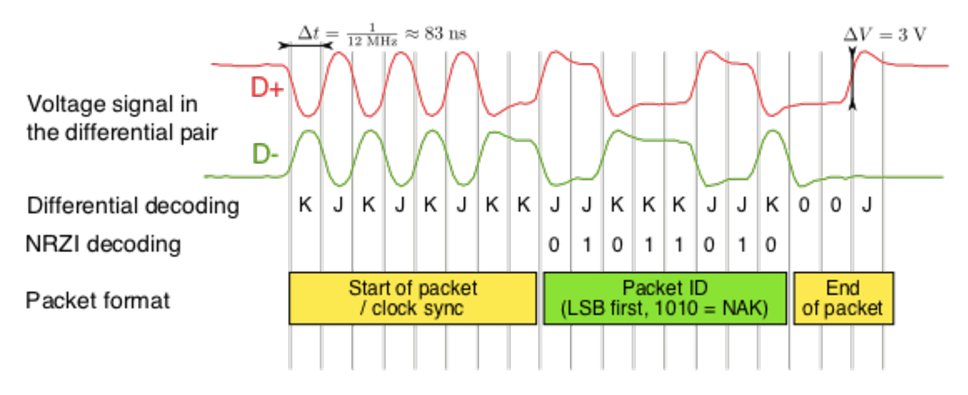
\includegraphics[width=14cm]{./Figures/serial/USB_signal_example.pdf}
  \rule{35em}{0.5pt}
  \caption[usb]{Exemple de signal USB}
  \label{fig:usb}
\end{figure}

L'interface USB est synchrone mais ne possède pas de ligne de clock. L'horloge est retrouvée à la réception grâce à une séquence d'entrainement de 8 bits. Une fois l'horloge synchronisée un packet ID (PID) est envoyé pour donner le type de message envoyé. Si le PID indique des données alors elles sont transmises. Finalement le paquet est terminé par une séquence "End of Packet" de trois bits.

D'un point de vue logiciel, l'interface USB s'accède grâce à un HAL ou par un pilote si il y a un système d'exploitation.

\section{Comparaisons et choix d'une interface}

\begin{table}[!htbp]
\begin{center}
{\fontfamily{phv}\selectfont
\begin{tabular}{|c|c|c|c|c|c|}
\hline 
Interface & Noeuds & Vitesse & Async/Sync & Duplex & Utilisation\\
\hline  
\hline 
RS-232C & 1 & 115kHz & A & Full & Terminal\\
\hline 
SPI & 1 à 5 & 100MHz & S & Full & Données\\
\hline
I2C & 256 & 1MHz & S & Half & Configuration\\
\hline
USB 2.0 & 1 & 480MHz & S & Half & External\\
\hline
\end{tabular}
}
\end{center}
\caption{Comparaisons entre les différentes interfaces séries \label{serial}}
\end{table}

\section{Cas du MSP430}

Le MSP430 dispose de toutes les interfaces discutées précédemment. Il s'agit donc de déterminer les registres de configuration propres à chaque interface puis de les paramétrer correctement.

Exemple de configuration d'une interface série asynchrone, style RS-232C:

\lstset{style=customc}
\begin{lstlisting}
UCA0CTL0 |= UCPEN | UCPAR;	//parity enabled, even, one stop(default), 8-bit (default), async (default)
UCA0CTL1 |= UCSSEL_2;		//SMCLK
UCA0BR0 = 0x09;				//115200 bauds selon table du fabriquant
UCA0BR1 = 0x00;
UCA0MCTL = 0x02;			//115200 bauds selon table du fabriquant		
 
UCA0IE |= UCRXIE | UCTXIE;	//Interrupt enable
	
P2DIR |= 0x01;				//P2.0 vers sortie 	 
 
#pragma vector=USCI_A0_VECTOR
__interrupt void usci_a0_isr(void)
{
  switch(__even_in_range(UCA0IV ,4))
  {
  case 0: 	break;
  case 2:
   	while (!(UCA0IFG & UCTXIFG));
	  UCA0TXBUF = UCA0RXBUF;
		break;
  case 4:
   	P2OUT ^= 0x01;		// toggle P2.0 avec exclusive-OR 
		break;
  default: 	break;
  }
}
\end{lstlisting}

L'interaction avec les registres de réception ou d'émission est effectuée par interruption dans ce cas ci. Le vecteur USCI\_A0\_VECTOR contient plusieurs sources d'interruptions possibles c'est pourquoi il faut les sélectionner à l'aide d'un switch case. Le "case 2" correspond à une réception et le "case 4" à une émission. Lors d'une réception on test si l'émission n'est pas active puis on copie le message reçu sur la sortie. C'est un relai qui allume une LED lorsque le message a été relayé.